
\subsection{Assembly}\label{section:assembly}
Assembly is a low-level programming language in which, generally speaking, each statement corresponds to one instruction executed by the CPU. Assembly statements are compiled into byte sequences of machine code called \emph{opcodes}.

An assembly statement starts with the name of the instruction (the \emph{mnemonic}), followed by its operands (i.e. arguments). \autoref{listing:assembly example} shows an assembly statement where \texttt{mov} is the mnemonic and \texttt{eax} and \texttt{1} are the operands.

\begin{lstlisting}[caption={A single instruction moving the integer \texttt{1} into the register \texttt{eax}.}, label={listing:assembly example}, captionpos=b]
mov eax, 1
\end{lstlisting}

x86 assembly code is written in either Intel syntax (mostly used for Windows development) or AT\&T syntax (mostly used for Linux development). As we focus on Windows in this thesis, we will use the Intel syntax style.

In this section, we will discuss some basic instructions. There are, however, many more instructions used to efficiently perform operations on specific data types.

\subsubsection{Arithmetic Instructions}
x86 provides instructions for basic arithmetic.

\begin{itemize}
    \item \texttt{add op0, op1}: Add the value of \texttt{op1} to \texttt{op0}.
    \item \texttt{sub op0, op1}: Subtract the value of \texttt{op1} from \texttt{op0}.
    \item \texttt{imul op0, op1}: Multiply the value of \texttt{op0} with \texttt{op1} and store the result in \texttt{op0}.
    \item \texttt{idiv op0}: Divide the contents of \texttt{edx:eax} (a 64-bit value of which the 32 most significant bits are taken from \texttt{edx} and the 32 least significant bits are taken from \texttt{eax}) by \texttt{op0} and store the result in \texttt{eax}.
    \item \texttt{inc op0}: Increase the value of \texttt{op0} by 1.
    \item \texttt{dec op0}: Decrease the value of \texttt{op0} by 1.
\end{itemize}

\subsubsection{Logical Instructions}
x86 provides instructions for logical operations.

\begin{itemize}
    \item \texttt{and op0, op1}: Compute the bitwise and \texttt{op0} and \texttt{op1} and store the result in \texttt{op0}.
    \item \texttt{or op0, op1}: Compute the bitwise or of \texttt{op0} and \texttt{op1} and store the result in \texttt{op0}.
    \item \texttt{xor op0, op1}: Compute the bitwise exclusive or of \texttt{op0} and \texttt{op1} and store the result in \texttt{op0}.
    \item \texttt{not op0}: Compute the bitwise not of \texttt{op0} and store the result in \texttt{op0}.
\end{itemize}

\subsubsection{Data Movement Instructions}
x86 provides instructions for moving data between memory and registers.

\begin{itemize}
    \item \texttt{mov op0, op1}: Move the data stored in \texttt{op1} into \texttt{op0}.
    \item \texttt{lea op0, op1}: Move the address (i.e. pointer) stored in \texttt{op1} into \texttt{op0}.
\end{itemize}

\subsubsection{Stack Instructions}
x86 provides instructions for manipulating the call stack.

\begin{itemize}
    \item \texttt{push op0}: Push \texttt{op0} to the stack. This decreases the stack pointer. As pushing data to the stack is essentially writing the data to memory, \texttt{push eax} is equivalent to \autoref{listing:push with mov}.

\begin{lstlisting}[caption={The \texttt{push eax} instruction written in terms of \texttt{sub} and \texttt{mov}.}, captionpos=b, label={listing:push with mov}]
sub esp, 4
mov [esp], eax
\end{lstlisting}

    \item \texttt{pop op0}: Pop the top element from the stack and store it in \texttt{op0}. This increases the stack pointer. \texttt{pop eax} is equivalent to \autoref{listing:pop with mov}.

\begin{lstlisting}[caption={The \texttt{pop eax} instruction written in terms of \texttt{mov} and \texttt{add}.}, captionpos=b, label={listing:pop with mov}]
mov eax, [esp]
add esp, 4
\end{lstlisting}

\end{itemize}

\subsubsection{Control Flow Instructions}\label{section:control flow instructions}
x86 also provides instructions to control the flow of a program. This allows for subroutines (i.e. functions) to be defined and called. It also allows for conditional branching.

\begin{itemize}
    \item \texttt{call op0}: Call a subroutine defined at \texttt{op0}.

    A \texttt{call} performs two operations:
    \begin{enumerate}
        \item It pushes the address after the \texttt{call} instruction to the stack (This is the \emph{return address}).
        \item It changes the \texttt{eip} to the address that is being called (i.e. the next instruction will be at the address that is being called).
    \end{enumerate}

    If \texttt{op0} is an address, the call is \emph{direct}, because the function that is being called is known at compile time or load time. If \texttt{op0} is a register, the call is \emph{indirect} as the address to the function that is called is determined at runtime.

    \item \texttt{ret}: Signal the end of a subroutine and return to the caller. It pops the return address from the stack and jumps to it.
    \item \texttt{jmp op0}: Jump to the instruction at \texttt{op0}.
    \item \texttt{cmp op0, op1} and conditional jumps: It is possible to only jump if a condition is met. The \texttt{cmp} instruction compares the values of its two operands and stores the result in the special \texttt{eflags} register. A conditional jump instruction (e.g. \texttt{je op0}, \texttt{jne op0} and \texttt{jge op0}) reads this result and jumps if its specific condition is met. For example, \texttt{je op0} jumps to \texttt{op0} when the operands of \texttt{cmp} are equal.
\end{itemize}

Because of the control-flow instructions, assembly code is not sequential, but rather a graph structure that can loop and skip code. The code between two control flow instructions is run sequentially and called a \emph{basic block}. This creates a \emph{control flow graph} of basic blocks and paths between these blocks. The conditionals in the code decide which paths are taken. \autoref{fig:control flow graph} shows an example of the control flow graph of a function.

\begin{figure}[ht]
    \centering
    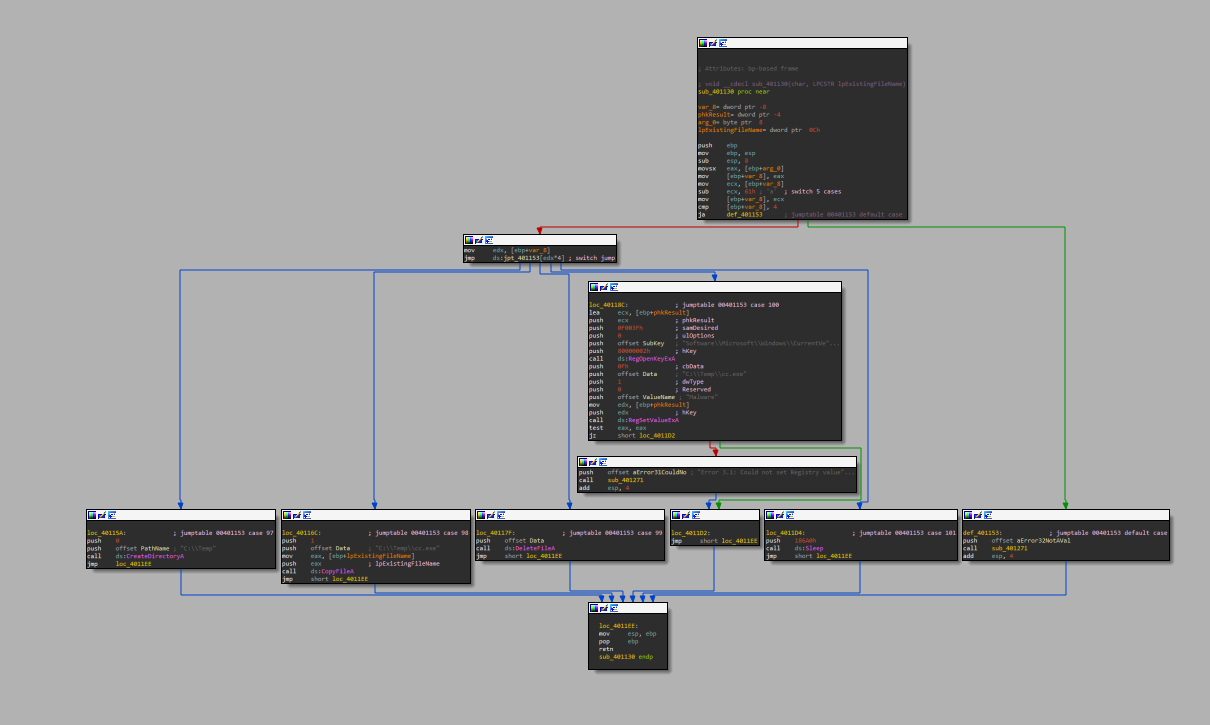
\includegraphics[width=0.9\textwidth]{resources/images/control_flow_graph.png}
    \caption{A screenshot from IDA Pro showing a control flow graph.}\label{fig:control flow graph}
\end{figure}
